
We know that equation of the line passing through given a point and a plane
\begin{equation}\label{eq:solutions/line_plane/107/eq2}
	\vec{r} = \vec{a}+\lambda\vec{m}
\end{equation}
Also we can find direction vector from the Cartesian form of equation
\begin{equation}
	\frac{x-x_1}{a} = \frac{y-y_1}{b} = \frac{z-z_1}{c}
\end{equation}
This can be expressed as
\begin{equation}
	\vec{x} = \myvec{x_1\\y_1\\z_1} + \lambda\myvec{a\\b\\c}
\end{equation}
where $\vec{a} = \myvec{x_1\\y_1\\z_1}$ is a point on given line and $\vec{m} = \myvec{a\\b\\c}$ is the direction vector.
\\
Distance between the point and point of intersection.
\begin{equation}
	D = \sqrt{(x2-x1)^2 + (y2-y1)^2 + (z2-z1)^2}
\end{equation}
Writing given equation (1.0.1) in vector form as
\begin{equation}
	\vec{x} = \myvec{2\\-1\\2} + \lambda\myvec{3\\4\\2}
\end{equation}
substitute (3.0.1) in (1.0.2)
to find the value of $\lambda$

\begin{equation}
	\myvec{1 & -1 & 1}\cbrak{\myvec{2 \\ -1 \\2} + \lambda \myvec{3\\4\\2}} = 5	
	\end{equation}
by multiplying the row vector with the first column vector 
\begin{equation}
 1(2) -1(-1) + 1(2) = 5
\end{equation}
by multiplying the row vector with the coefficient column vector of lambda 
\begin{equation}
 1(3\lambda) -1(4\lambda) +1(2\lambda) = \lambda
\end{equation}
we get as
\begin{equation}
\lambda = 0
\end{equation}
The line intersects the plane at
\begin{equation}
 \vec{x}_0 = \myvec{2\\-1\\2}
\end{equation}
Finally the distance between the point 
$\vec{P} = \myvec{-1\\-5\\-10}$ and intersection point $\vec{x}_0 = \myvec{2\\-1\\2}$ is

\begin{equation}
 \norm{x_0-P}=\sqrt{(2+1)^2+(-1+5)^2+(2+10)^2}
\end{equation}

\begin{equation}
 \norm{x_0-P}=13	
\end{equation}
\begin{figure}[h]
	\centering
	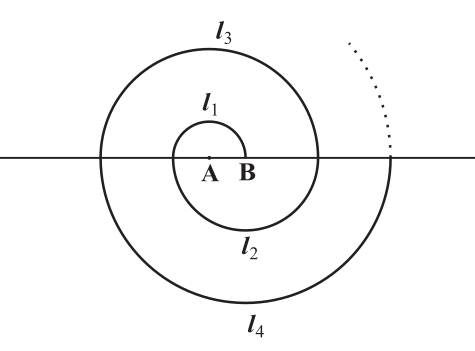
\includegraphics[width=\columnwidth]{./solutions/line_plane/107/fig.png}
	\caption{Equation of line passing through point $x_0$ and intersection to line (1.0.1)}
	\label{eq:solutions/line_plane/107/fig:}
\end{figure}

